\subsection{Some results in Adaptive Data Analysis}
%\wq{I think we can move this subsection into appendix. Maybe just leave theorm 1.2 and 1.3}
%\jl{I don't agree}
In Adaptive Data Analysis an \emph{analyst} is interested in studying some distribution $\dist$ over some domain $\univ$.  Following previous works~\cite{DworkFHPRR15,HardtU14,BassilyNSSSU16}, we focus on the setting where the analyst is interested in answers to \emph{statistical queries} (also known as \emph{linear queries}) over the distribution.  A statistical query is usually defined by some function $\qquery \from \univ \to [-1,1]$ (often other codomains such as $[0,1]$ or $[-R,+R]$, for some $R$, are considered).  The analyst wants to learn the \emph{population mean}, which is defined as 
$\qquery(\dist) = \ex{\sample \sim \dist}{\qquery(\sample)}$. 
%
We assume that the distribution $\dist$ can only be accessed via a set of \emph{samples} $\sample_1,\dots,\sample_n$ drawn independently and identically distributed (i.i.d.) from $\dist$.  These samples are held by a mechanism $\mech(\sample_1,\dots,\sample_n)$ who receives the query $\query$ and computes an answer 
$\answer \approx \qquery(\dist)$.
%
The na\"ive way to approximate the population mean is to use the \emph{empirical mean}, which (abusing notation) is defined as 
$\qquery(\sample_1,\dots,\sample_n) = \frac{1}{n} \sum_{i=1}^{n} \qquery(X_i)$.
However, the mechanism $M$ can adopt some methods for improving the generalization error $| a- \qquery(\dist)|$.

In this work we consider analysts that ask a sequence of $k$ queries $\qquery_1,\dots,\qquery_k$.  If the queries are all chosen in advance, independently of the answers $a_1,\dots,a_k$ of each other, then we say they are \emph{non-adaptive}.  If the choice of each query $\qquery_j$ depends on the prefix $\qquery_1,\answer_1,\dots,\qquery_{j-1},\answer_{j-1}$ then they are \emph{fully adaptive}.  An important intermediate notion is \emph{$\qrounds$-round adaptive}, where the sequence can be partitioned into $\qrounds$ batches of non-adaptive queries.  Note that non-adaptive queries are $1$-round and fully adaptive queries are $k$-round adaptive.

We now review what is known about the problem of answering $r$-round adaptive queries.  
\begin{thm}[\cite{BassilyNSSSU16}] 
\label{thm:nonadapt-adapt}
\begin{enumerate}

\item For any distribution $\dist$, and any $k$ \emph{non-adaptive} statistical queries, with high probablity,
% $$
$
\max_{j=1,\dots,k} | \answer_j - \qquery_j(\dist) | = O\left( \sqrt{\frac{\log k}{n}}  \right)
% $$
$.
%
\item For any distribution $\dist$, and  any $k$  \emph{$\qrounds$-round adaptive} statistical queries, with $\qrounds \geq 2$, with high probablity, the empirical mean (rounded to an appropriate number of bits of precision)\footnote{With infinite precision even two queries may give unbounded error, when the first query's result encodes the whole data.} satisfies:\\
% $$
$
\max_{j=1,\dots,k} | \answer_j - \qquery_j(\dist) | = O\left( \sqrt{\frac{k}{n}}  \right)
% $$
$
\end{enumerate}
\end{thm}
In fact, these bounds are tight (up to constant factors) which means that even allowing one extra round of adaptivity leads to an exponential increase in the generalization error, from $\log k$ to $k$.

\citet{DworkFHPRR15} and \citet{BassilyNSSSU16} showed that by using carefully calibrated Gaussian noise in order to limit the dependency of a single query on the specific data instance, one 
can actually achieve much stronger generalization error as a function of the number of queries, specifically.
\begin{thm}[\cite{DworkFHPRR15, BassilyNSSSU16}] \label{thm:gaussiannoise} For any distribution $\dist$, any $k$, any $\qrounds \geq 2$ and any \emph{$\qrounds$-round adaptive} statistical queries, if we answer queries with carefully calibrated Gaussian noise, with high probablity,  we have:
\begin{center}
  $
\max_{j=1,\dots,k} | \answer_j - \qquery_j(\dist) | = O\left( \frac{\sqrt[4]{k}}{\sqrt{n}}  \right)
$  
\end{center}
\end{thm}
% Notice that in order to Theorem~\ref{thm:gaussiannoise} has different quantification in that the optimal choice of mechanism depends on the number of queries.  Thus, we need to know the number of queries \emph{a priori} to choose the best mechanism.
More interestingly, \citet{DworkFHPRR15}
also gave a refined bounds that can be achieved with different mechanisms depending on the number of rounds of adaptivity.   \begin{thm}[\cite{DworkFHPRR15}] \label{thm:gaussiannoise2} For any $r$ and $k$, there exists a mechanism such that for any distribution $\dist$, and any $\qrounds \geq 2$ any \emph{$\qrounds$-round adaptive} statistical queries, with high probablity, it satisfies
\begin{center}
  $
\max_{j=1,\dots,k} | \answer_j - \qquery_j(\dist) | = O\left( \frac{r \sqrt{\log k}}{\sqrt{n}}  \right)
$  
\end{center}
\end{thm}
Notice that Theorem~\ref{thm:gaussiannoise2} has different quantification in that the optimal choice of mechanism depends on the number of queries {and number of rounds of adaptivity}.  This suggests that if one knows a good \emph{a priori upper bound on the number of rounds of adaptivity}, one can choose the appropriate mechanism and get a much better guarantee in terms of the generalization error.
As an example, as we can see in Fig.~\ref{fig:generalization_errors}, if we know that an algorithm is 2-rounds adaptive, we can choose data splitting as {the} mechanism, while if we know that an algorithm has many rounds of adaptivity we can choose Gaussian noise. It is worth to stress that by knowing the number of rounds of adaptivity one can also compute a concrete upper bound on the generalization error of a data analysis. This information allows one to have a quantitative, a priori, estimation of the effectiveness of a data analysis. 
This motivates us to design a static program analysis aimed at giving good \emph{a priori} upper bounds on the number of rounds of adaptivity of a program. 

{\small
\begin{figure}
\centering
\begin{subfigure}{.2\textwidth}
\begin{centering}
$
    \begin{array}{l}
    \kw{towRounds(k)} \triangleq \\
           \clabel{ \assign{a}{0}}^{0} ;
            \clabel{\assign{j}{k} }^{1} ; \\
            \ewhile ~ \clabel{j > 0}^{2} ~ \edo ~ \\
            \Big(
             \clabel{\assign{x}{\query(\chi[j] \cdot \chi[k])} }^{3}  ; \\
             \clabel{\assign{j}{j-1}}^{4} ;\\
            \clabel{\assign{a}{x + a}}^{5}       \Big);\\
            \clabel{\assign{l}{\query(\chi[k]*a)} }^{6}\\
        \end{array}
$
\caption{}
\end{centering}
\end{subfigure}
\begin{subfigure}{.4\textwidth}
%}
\qquad
\begin{centering}
\begin{tikzpicture}[scale=\textwidth/16cm,samples=250]
\draw[] (0, 10) circle (0pt) node
{{ $a^0: {}^{\lambda \trace_0. 1}_{0}$}};
\draw[] (0, 7) circle (0pt) node
{\textbf{$x^3: {}^{\lambda \trace_0. \env(\trace_0) k}_{1}$}};
\draw[] (0, 4) circle (0pt) node {{ $a^5: {}^{\lambda \trace_0. \env(\trace_0) k}_{0}$}};
\draw[] (0, 1) circle (0pt) node
{{ $l^6: {}^{\lambda \trace_0. 1}_{1}$}};
% Counter Variables
\draw[] (8, 9) circle (0pt) node {\textbf{$j^1: {}^{\lambda \trace_0. 1}_{0}$}};
\draw[] (8, 6) circle (0pt) node {{ $j^4: {}^{\lambda \trace_0. \env(\trace_0) k}_{0}$}};
%
% Value Dependency Edges:
\draw[ ultra thick, -latex, densely dotted,] (0, 1.5)  -- (0, 3.5) ;
\draw[ ultra thick, -latex, densely dotted,] (0, 4.5)  -- (0, 6.5) ;
\draw[ thick, -latex] (0, 4.5)  to  [out=-230,in=230]  (0, 9.5) ;
\draw[ thick, -Straight Barb] (1.5, 3.8) arc (120:-200:1);
\draw[ thick, -Straight Barb] (9, 6.5) arc (150:-150:1);
\draw[ thick, -latex] (8, 6.5)  -- (8, 8.5) ;
\draw[ thick, -latex] (0, 1.5)  to  [out=-230,in=230]  (0, 9.5) ;
% Control Dependency
\draw[ thick,-latex] (2, 7)  -- (6, 9) ;
\draw[ thick,-latex] (2, 4.5)  -- (6, 9) ;
\draw[ thick,-latex] (2, 7)  -- (6, 6) ;
\draw[ thick,-latex] (2, 4.5)  -- (6, 6) ;
\end{tikzpicture}
\caption{}
\end{centering}
\end{subfigure}
   \begin{subfigure}{.36\textwidth}
   \begin{centering}
   \begin{tikzpicture}[scale=\textwidth/18cm,samples=200]
\draw[] (0, 10) circle (0pt) node
{{ $a^0: {}^1_{0}$}};
\draw[] (0, 7) circle (0pt) node
{\textbf{$x^3: {}^{k}_{1}$}};
\draw[] (0, 4) circle (0pt) node
{{ $a^5: {}^{k}_{0}$}};
\draw[] (0, 1) circle (0pt) node
{{ $l^6: {}^{1}_{1}$}};
% Counter Variables
\draw[] (5, 9) circle (0pt) node {\textbf{$j^1: {}^{1}_{0}$}};
\draw[] (5, 6) circle (0pt) node {{ $j^4: {}^{k}_{0}$}};
%
% Value Dependency Edges:
\draw[ ultra thick, -latex, densely dotted,] (0, 1.5)  -- (0, 3.5) ;
\draw[ ultra thick, -latex, densely dotted,] (0, 4.5)  -- 
% node [left] {\highlight{$\trace_0 \to \env(\trace_0) k $}}
(0, 6.5) ;
\draw[ thick, -latex] (0, 4.5)  to  [out=-230,in=230]  
% node [left] {\highlight{$\trace_0 \to \env(\trace_0) k $}}
(0, 9.5) ;
\draw[ thick, -Straight Barb] (1.5, 3.5) arc (120:-200:1);
\draw[ thick, -Straight Barb] (6.5, 6.5) arc (150:-150:1);
    % The Weight for this edge
    % \draw[](9, 6) node [] {\highlight{$\trace_0 \to \env(\trace_0) k  $}};
\draw[ thick, -latex] (5, 6.5)  -- (5, 8.5) ;
% Control Dependency
\draw[ thick,-latex] (1.5, 7)  -- (4, 9) ;
\draw[ thick,-latex] (1.5, 4)  -- (4, 9) ;
\draw[ thick,-latex] (1.5, 7)  -- (4, 6) ;
\draw[ thick,-latex] (1.5, 4)  -- (4, 6) ;
\draw[ thick, -latex] (0, 1.5)  to  [out=-230,in=230]  (0, 9.5) ;
\end{tikzpicture}
\caption{}
   \end{centering}
   \end{subfigure}
\vspace{-0.4cm}
 \caption{(a) The program $\kw{towRounds(k)}$, an example 
%  of a program 
with two rounds of adaptivity (b) The corresponding execution-based dependency graph (c) The program-based dependency graph from $\THESYSTEM$.
}
\label{fig:overview-example}
% \vspace{-0.8cm}
\end{figure}
}


\subsection{ {\THESYSTEM} formally through an example.}
We illustrate the key technical components of our framework through a simple adaptive data analysis with two rounds of adaptivity.
% They are 1. the query while language for expressing a data analysis formally, 2. the definition of \emph{adaptivity} (\emph{adaptivity} is the short for \emph{rounds of adaptivity} used in the rest of the paper) based on the language semantics, and 3. the static analysis algorithm providing a sound upper bound on a data analysis' adaptivity.
% }
% \detailed{
% In "two rounds strategy" analysis, the analyst asks in total $k+1$ queries to the mechanism in two phases, the symbol $k$ is an input from the data analyst of this strategy and has no limit on the kind, which can be a constant, or a symbol or even an expression such as $(k+3)*2$.
% } 
%
In this analysis, an analyst asks $k+1$ queries to a mechanism in two phases.
In the first phase, the analyst asks $k$ queries and stores the answers that are provided by the mechanism. In the second phase, the analyst constructs a new query based on the results of the previous $k$ queries and sends this query to the mechanism. 
The mechanism is abstract here and our goal is to use static analysis to provide an upper bound on adaptivity to help choose the mechanism.
This data analysis assumes that the data domain $\univ$ 
contains at least $k$ numeric attributes 
(every query in the first phase focuses on one), which we index just by natural numbers.
The implementation of this data analysis in the language of {\THESYSTEM} is presented in Fig.~\ref{fig:overview-example}(a).

The {\THESYSTEM} language extends a standard while language\footnote{Programs components are labeled, so that we can uniquely identify every component.} with a query request constructor denoted $\query$.
 Queries have the form $\query(\qexpr)$, where $\qexpr$ is a special expression (see syntax in Section~\ref{sec:loop_language}) 
representing a function $\from \univ \to U$ on rows of an hidden database that is only accessible through the mechanisms. The domain $\univ$ of this function is the (arbitrary) domain of rows of the database. The codomain $U$ of this function is the query output space which, depending on the specific program, could be $[-1,1]$, $[0,1]$ or $[-R,+R]$, for some $R$. We use this formalization because we are interested in linear queries which, as we discussed in the previous section, compute the empirical mean of functions on rows.
 As an example, $x \leftarrow \query(\chi[j] \cdot \chi[k])$ computes an approximation, according to the used mechanism, of the empirical mean of the product of the $j^{th}$ attribute and $k^{th}$ attribute, identified by $\chi[j] \cdot \chi[k]$. Notice that we don't materialize the mechanism but we assume that it is implicitly run when we execute the query. 
 In Fig.~\ref{fig:overview-example}(a), the queries inside the while loop correspond to the first phase of the data analysis and compute the sum of the empirical mean of
the product of the $j$th attribute with the $k$th attribute. 
The query outside the loop corresponds to the second phase and computes an approximation of the empirical mean of the last attribute weighted by the sum of the empirical mean of the first $k$ attributes.


This example is intuitively 2-rounds adaptive since we have two clearly distinguished phases, and the queries that we ask in the first phase do not depend on each other (the query $\chi[j] \cdot \chi[k]$ at line $3$ only relies on the counter $j$ and input $k$), while the last query 
(at line 6) depends on the results of all the previous queries. 
However, capturing this concept formally is surprisingly challenging. The difficulty comes from the quantitative nature of this concept and how this quantitative nature interacts with data and control dependency. We describe how we capture it next. 
% \mg{this is weaker than it was in the previous submission.}

%%%%%%%%%%%%%%%%%%%%%%%%%%%%%%%%%%%Some details that might be useful when make passes %%%%%%%%%%%%%%%%%
% \jl{ The $\bullet$ stands for no query, for instance, the second event in the trace $(j, 1, \env(\trace)k , \bullet) $ tells us the assignment at line $1$ does not request a query.} \jl{The third event is a testing event corresponding to the guard of the while loop at line $2$. The evaluation of the query request in the second phase is tracked in }
% % \jl{ 
% The $\bullet$ is a default value for non-query event, 
% for instance, the second event in the trace $(j, 1, K , \bullet) $ tells us the assignment at line $1$ does not request a query.
% The third event is a testing event corresponding to the guard of the while loop at line $2$. The evaluation of the query request in the second phase is tracked in 
% % }
\subsubsection{Adaptivity definition}
\label{sec:adaptivity-informal}
%%%%%%%%%%%%%%%%%%%%%%%%%%%%%%%%%%% Details Below that might be useful when make passes %%%%%%%%%%%%%%%%%
% \detailed{To formally define the adaptivity, we build a directed graph representing the possible dependencies between queries of a program and we call this graph: execution-based dependency graph. The vertices represent the assigned program variables and the edges satisfy the dependency relations between vertices.   Fig.~\ref{fig:overview-example}(b) is the execution dependency graph we build based on the "two rounds strategy program" in Fig.~\ref{fig:overview-example}(a). In brief, the graph is built by collecting the assigned variables with labels of the target program as vertices, which are $a^0$, $j^1$,...$a^5$,$l^6$. We check if there is an edge between two vertices by our dependency relation over two labeled variables (defined in Section~\ref{sec:dep_adaptivity} ). This dependency relation relies on the execution of the program recorded by a trace generated by our trace semantics, which is the reason we call this graph "execution-based". 
% Intuitively from Fig.~\ref{fig:overview-example}(a), the query in the second phase (at line 6) depends on the query results in the first phase stored in $a$ at line 5, and the variable $a$ also relies on the queries at line 3. Correspondingly, we have two edges $(l^6, a^5)$ and $(a^5, x^3)$ in our execution-based dependency graph in Fig.~\ref{fig:overview-example}(b). Besides, we also have special edge which is a circle, to track any variable being updated with its previous value recursively. For instance, the counter $j$ and the variable $a$ are updated based on previous values $k$ times in the first phase and we see two circle edges on $a^5$ and $j^4$.}

The central property we are after in this work is the \emph{adaptivity of a program}. We define formally this notion in three steps, which we will describe in details in Section~\ref{sec:adaptivity}. First, we define a notion of dependency, or better \emph{may-dependency}, between variables. To do this we take inspiration from previous works on dependency analysis and information flow control and we say that a variable \emph{may depend} on another one if changing the execution of the latter can affect the execution of the former. 
We can see in Fig.~\ref{fig:overview-example}(a) that the value of the variable $l$, which corresponds to the result of the execution of the query in the second phase (in the command with label 6), is affected by the value of the variable $x$, which corresponds to the result of the execution of the query at line 3 in the first phase, via the variable $a$.
To formally define this notion of dependency, as in information flow control, we use the execution history of programs recorded by a trace semantics (see Definition~\ref{def:var_dep}).
% \mg{Please, double check that I refer to the right definition. }  

Second, we build an annotated weighted directed graph representing the possible dependencies between labeled variables. We call this graph \emph{semantics-based dependency graph} to stress that this graph summarizes the dependencies we could see if we knew the overall behavior of the program. 
The vertices of the graph are the assigned program variables with the label of their assignments, edges are pairs of labeled variables which satisfy the dependency relations, weights are functions associated with vertices and describe the number of times the assignment corresponding to the vertex is executed when the program is run in a given starting state\footnote{In our trace semantics the state is recorded in the trace, so an initial state is actually represented by an initial trace. We will use this terminology in later sections.}, and the annotations, which we call \emph{query annotations}, are bits associated with vertices and describe if the corresponding assignment comes from a query (1) or not (0).
The \emph{semantics-based dependency graph} of the $\kw{twoRounds(k)}$ program
we gave in Fig.~\ref{fig:overview-example}(a) is described in Fig.~\ref{fig:overview-example}(b) (we use dashed arrows for two edges that will be highlighted in the next step, for the moment these can be considered similar to the other edges---i.e. solid arrows). We have all the variables that are assigned in the program with their labels, and edges representing dependency relations between them. 
For example, we have two edges $(l^6, a^5)$ and $(a^5, x^3)$ describing the dependency between the variables assigned by queries. The vertices $l^6$ and $x^3$ are the only ones with query annotation $1$ (the subscript), since they are the only two variables that are in assignments involving  queries. Notice that the graph contains cycles---in this example it contains two self-loops. These cycles capture the fact that the variables $a^5$ and $j^4$ are updated at every iteration of the loop using their previous values. Cycles are essential to capture mutual dependencies like the ones that are generated in loops. Adaptivity is a quantitative notion, so capturing this form of dependencies is not enough. This is why we also use weights. The weight of a vertex is a function that given an initial state returns a natural number representing 
the number of times the assignment corresponding to a vertex is visited during the program execution starting in this initial state.  
For example, the vertex $l^{6}$ has weight {$\lambda \trace.1$} since for every initial state {$\trace$} the corresponding assignment will be executed one time, the vertex $a^5$ on the other hand has weight {$\lambda \trace. \env(\trace) k$ since the corresponding assignment will be executed a number of times that correspond to the value of $k$ in the initial state $\trace$, and $\env$ is the operator reading value of $k$ from $\trace$.
}

% It is a function which takes an initial state, $\trace_0$ as input,
% then executes the program, and counts the evaluation times of the query request $\clabel{\assign{l}{\query(\chi[k]*a)} }^{6}$ during the execution.
% % returns $1$ for every starting state, since 
% Since this query at line $6$ is outside of any loop, we are expecting this function always return the count $1$ given any initial state.
% The query annotation of this vertex is $1$, which  indicates that 
% $\clabel{\assign{l}{\query(\chi[k] * a)}}^6$ is a query request.
% For another vertex, $a^{5}:{}^{w_{a^{5}}}_0$ in the while loop, we expect its weight function
% returns different counts if the input initial traces have different initial value for $k$.
% Because $\clabel{\assign{a}{x + a}}^{5}$ will be executed different times if the input $k$  is different.
% Its subscript $0$ representing this is a non-query assignment.



% Besides, we also have special edge which is a circle, to track any variable being updated with its previous value recursively. 
% For instance, the loop counter $j$ and the variable $a$ are updated based on previous values $k$ times in the first phase and we see two circle edges on $a^5$ and $j^4$.

%%%%%%%%%%%%%%%%%%%%%%%%%%%%%%%%%%% Details Below that might be useful when make passes %%%%%%%%%%%%%%%%%
% \detailed{The existence of circle edge \jl{(there isn't a name 'circle edge', the terminology is cycle)}
%  allows our graph to express situation when a variable relies on its previous value recursively inside a while loop, but not show how many times of this reliance, which is necessary to define adaptivity. For instance, if we modify our two round example a little bit to make the query $query(\chi[j]\dot \chi[k])$ at line $3$ relies on its previous result to $query(\chi[j]\dot\chi[k] + x)$, then intuitively its adaptivity becomes $k+1$. To this end, we add quantitative information to our graph: weight on every vertex.
% The weight of a vertex is a function that given a starting state returns a natural number representing 
% the number of times the vertex is visited when the program is executed starting from this state.}
% \jl{The existence of cycle
%  allows our graph to handle the while loop.
% When the variable in a while loop relies on its value in the previous iterations, the cycle expresses this reliance.
% But it cannot express the times of this reliance.
% For instance, if we modify the command $3$
% of the $\kw{twoRounds(k)}$ example
% into $\clabel{\assign{x}{\query(\chi[j] \cdot \chi[k] + x)}}^3$. 
% Then $x$ in every iteration relies on the result in the previous iteration
% and the intuitive adaptivity becomes $k+1$. But we don't know the number $k$ by only constructing the edge $x^3 \to x^3$.
% To this end, we add quantitative information to our graph: weight on every vertex.
% The weight of a vertex is a function that given a starting state returns a natural number representing 
% the number of times the vertex is visited during the program execution.
% }
% Each vertex in this graph has a superscript representing its weight, and a subscript $1$ or $0$ telling if the vertex corresponds to a query or not. We will call this subscript a query annotation. 
% For example, in Fig.~\ref{fig:overview-example}(b), the vertex $l^{6}:{}^{w_1}_1$, 
% has weight $w_1$, a constant function which returns $1$ for every starting state, since 
% this query at line $6$ is at most executed once regardless of the initial trace.
% The query annotation of this vertex is $1$, which  indicates that 
% $\clabel{\assign{l}{\query(\chi[k] * a)}}^6$ is a query request.
% Another vertex, $x^{3}:{}^{w_k}_1$, appears in the while loop. 
% It has as weight a function $w_k$ that for every initial state returns the value that $k$ has in this state, since this is also the number the while loop will be iterated. 
% The node $j^{4}:{}^{w_k}_0$ has as a subscript $0$ representing a non-query assignment.
% \jl{
% For example, in Fig.~\ref{fig:overview-example}(b), the vertex $l^{6}:{}^{w_{l^{6}}}_1$, 
% has weight ${w_{l^{6}}}$. It is a function which takes an initial state, $\trace_0$ as input,
% then executes the program, and counts the evaluation times of the query request $\clabel{\assign{l}{\query(\chi[k]*a)} }^{6}$ during the execution.
% % returns $1$ for every starting state, since 
% Since this query at line $6$ is outside of any loop, we are expecting this function always return the count $1$ given any initial state.
% The query annotation of this vertex is $1$, which  indicates that 
% $\clabel{\assign{l}{\query(\chi[k] * a)}}^6$ is a query request.
% For another vertex, $a^{5}:{}^{w_{a^{5}}}_0$ in the while loop, we expect its weight function
% returns different counts if the input initial traces have different initial value for $k$.
% Because $\clabel{\assign{a}{x + a}}^{5}$ will be executed different times if the input $k$  is different.
% Its subscript $0$ representing this is a non-query assignment.
%
%It has as weight a function $w_k$ that for every initial state returns the value that $k$ has in this state, since this is also the number the while loop will be iterated. 
% The node $j^{4}:{}^{w_k}_0$ has as a subscript $0$ representing a non-query assignment.
% }
%%%%%%%%%%%%%%%%%%%%%%%%%%%%%%%%%%% Details Below that might be useful when make passes %%%%%%%%%%%%%%%%%
% \detailed{Since the edges between two vertices represent the fact that one program variable may depend on the other,
% we can define the program adaptivity with respect to a initial trace by means of a walk traversing the graph, visiting each vertex no more than its weight with respect to the initial trace, and visiting as many query nodes as possible.
% Still, look again at our example, we can see that
% in the walk along the dotted arrows,  $l^{6} \to a^5 \to x^3 $, there are $2$ vertices with query annotation $1$ and that this number is maximal, i.e. we cannot find another walk having more than $2$ vertices with query annotation $1$, under the assumption that $k \geq 1$. So the adaptivity of the program in Fig.~\ref{fig:overview-example}(a)  is $2$,
% as expected.
% }
Third, we can finally define adaptivity using the semantics-based dependency graph. We actually define this notion with respect to an initial state $\tau$, since different states can give very different adaptivities.  
We consider 
% the longest walk  that visits each vertex $v$ of the semantics-based dependency graph no more than the value that the weight $w_v$ assign to $\tau$, and visits as many query nodes as possible. 
any  walk  that visits a vertex $v$ of the semantics-based dependency graph no more than the value that the vertex's weight $w_v$ associates to the initial state $\tau$, and that visits a maximal number of query vertices.
The number of query vertices visited is the adaptivity of the program with respect to $\tau$.
Looking again at Fig.~\ref{fig:overview-example}(b), and assuming that $\tau(k) \geq 1$, we can see that the 
walk along the dashed arrows,  $l^{6} \to a^5 \to x^3 $ has two vertices with query annotation $1$, and we cannot find another walk having more than $2$ query vertices, although there is another walk, $l^{6} \to x^3 $, which has $2$ query vertices. So the adaptivity of the program in Fig.~\ref{fig:overview-example}(a) with respect to $\tau$ is $2$. If we consider an initial state $\tau$ such that $\tau(k)=0$ we have that the adaptivity with respect to $\tau$ is instead $1$. 
%%%%%%Gap: %%%%%%%%%%%%%%%%%%%%%%%%%%%%%%%%%%%%%%%%%%%%%%%%%%%%%%%%%%%%%%%%%%%%%%%%%%%%%%%%%%%%%%%%%%%%%%%%%%%%%%%%%%%%%%%%%%%%%%%%%%%%%%%%%%%%%%%
% \begin{figure}
%     \centering   
%     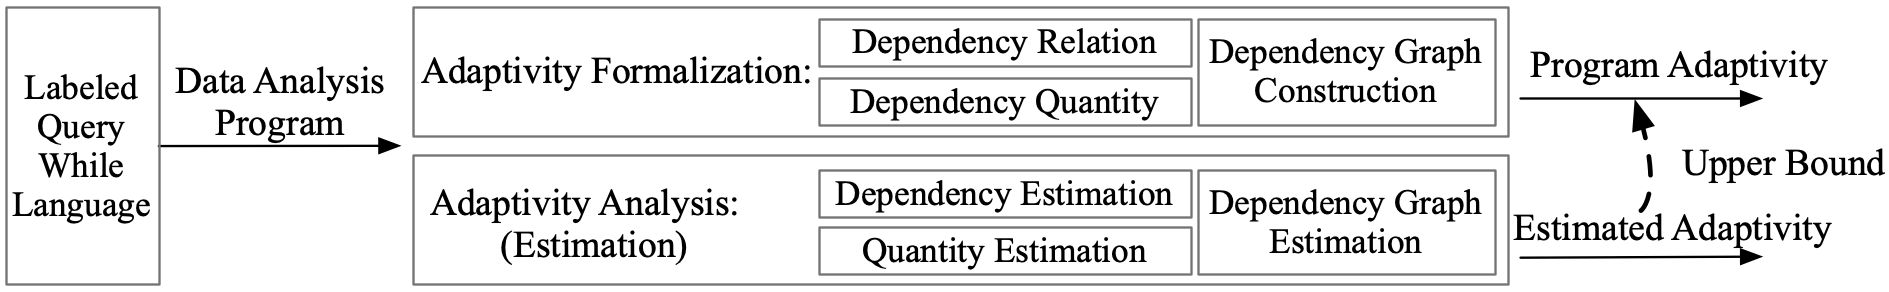
\includegraphics[width=1.0\textwidth]{architecture.png}
%     \vspace{-0.8cm}
%   \caption{High level architecture}
%     \label{fig:structure}
%     \vspace{-0.6cm}
% \end{figure}

\subsubsection{Static analysis}
%%%%%%%%%%%%%%%%%%%%%%%%%%%%%%% Previous Version Below that might be useful when make passes %%%%%%%%%%%%%%%%%
%  \detailed{The definition of adaptivity comes from the aforementioned execution-based dependency graph, 
%  our static analysis statically provides a sound upper bound on this adaptivity, via constructing another weighted graph, we call it estimated dependency graph. The upper bound is then found by searching a sound path with respect to our adaptivity in the generated graph. Different from the execution-based dependency which needs the trace from the execution, estimated one is built by our static analysis algorithm which takes the program itself as input. In brief, our algorithm is consist of a graph-generation algorithm, a weight computation algorithm and finally a path searching algorithm in the generated weighted graph.
%  }
%%%%%%%%%%%%%%%%%%%%%%%%%%%%%%% Previous Version Below that might be useful when make passes %%%%%%%%%%%%%%%%%
% \todo{In order to have a sound and accurate upper bound on the  adaptivity of a program $c$,
% we design a program analysis framework named {\THESYSTEM}.
% This framework composes two algorithms as shown in the double-stroke box and the dashed box in Fig.~\ref{fig:adaptfun}.
% The first algorithm in the double-stroke box combines the quantitative and dependency analysis techniques.
% It produces an estimated \emph{dependency graph} for a program.
% The second algorithm in the dashed box is a walk length estimation algorithm.
% It computes the upper bound on the program's \emph{adaptivity} over the estimated graph.}
% \jl{Since the definition of adaptivity comes from the aforementioned execution-based dependency graph, 
%  our static analysis statically provides a sound upper bound on this adaptivity via approximating this graph. The estimated graph is called \emph{estimated dependency graph}. 
%  The upper bound is then computed by searching the walk in this graph such that it can give a sound bound on the adaptivity.
%  Different from the execution-based dependency graph, the estimated one is produced by our static anlaysis algorithm, which only takes the program as input and does not rely on the execution history.
%  In brief, our algorithm is consist of a weighted graph-generation algorithm and a adaptivity computation algorithm over the graph.
%  }
 
 %%%%%%%%%%%%%%%%%%%%%%%%%%%%%%% Previous Version Above for Reference  %%%%%%%%%%%%%%%%%
To compute statically a sound and accurate upper bound on the \emph{adaptivity} of a program $c$,
we design a program analysis framework named {\THESYSTEM} which we will describe formally in Section \ref{sec:algorithm}. 
The structure of {\THESYSTEM} (Fig.~\ref{fig:adaptfun}) reflects in part the definition of adaptivity we discussed in the previous section. Specifically, {\THESYSTEM} is composed by two algorithms (the ones in dashed boxes in the figure), one for building a dependency graph, which we call \emph{estimated dependency graph}, and the other to estimate the adaptivity from this graph.  
The first algorithm generates the \emph{estimated dependency graph} using several program analysis techniques. Specifically,
 {\THESYSTEM} extracts the vertices and the query annotations by looking at the assigned variables of the program, it estimates the edges by using control flow and data flow analysis, and it estimates the weights by using symbolic reachability-bound analysis---weights in this graph are symbolic expressions over input variables. 
% This combined analysis allow us to obtain more accurate upper bounds than what we would obtain by using any of these single analysis technique in isolation.
The second algorithm estimates the
% longest 
walk which respects the weights and which visits the maximal number of query vertices.
%  as possible. 
The two algorithms together gives us an  upper bound on the program's \emph{adaptivity}.

 \begin{figure}
  \centering    
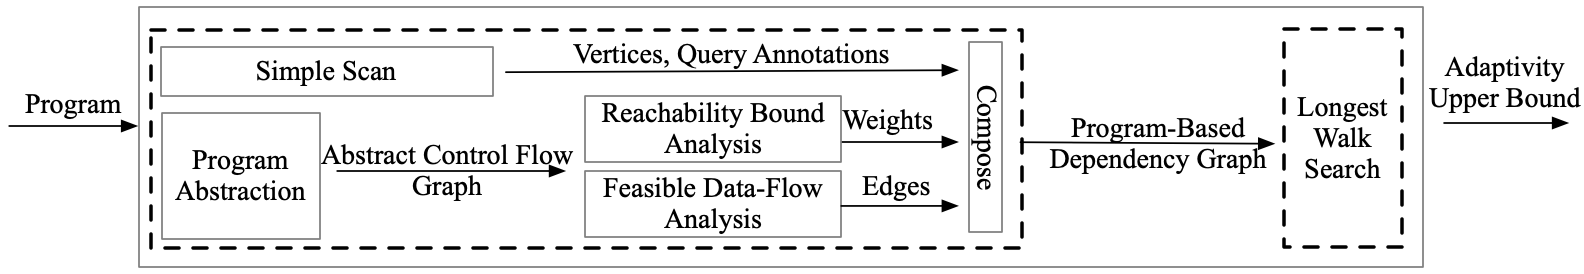
\includegraphics[width=1.0\columnwidth]{adapfun.png}
  \vspace{-0.8cm}
  \caption{The overview of {\THESYSTEM}}
  \label{fig:adaptfun}
  \vspace{-0.5cm}
\end{figure}

 
%%%%%%%%%%%%%%%%%%%%%%%%%%%%%%%%%%% Details Below that might be useful when others are making passes %%%%%%%%%%%%%%%%%
%   \detailed{Fig.~\ref{fig:overview-example}(c) is the resulting estimated graph of our static analysis algorithm which consumes the program in Fig.~\ref{fig:overview-example}(a).The edges are generated by our graph generation algorithm which combines control flow analysis and data flow analysis, presented in Section~\ref{sec:alg_edgegen}). We can easily see the generated graph in Fig.~\ref{fig:overview-example}(c) is a safe approximation of its execution-based counterpart in Fig.~\ref{fig:overview-example}(b), in the way that we can find a corresponding edge in Fig.~\ref{fig:overview-example}(c) for all the edges in Fig.~\ref{fig:overview-example}(b). We call the weight of every vertex computed by our algorithm as estimated weight,  }
%   estimated by using a reachability-bound estimation algorithm (presented in Section~\ref{sec:alg_weightgen}). \detailed{Different from the execution-based weight $w_1$ or $w_k$ in Fig.~\ref{fig:overview-example}(b) which is a function whose output relies on the initial trace, our estimated weight} can be symbolic and provide a sound upper bound on its execution-based weight of the corresponding vertex in the execution-based dependency graph. For instance, 
%   the estimated weight $k$ of the vertex $x^{3}$ in Fig.~\ref{fig:overview-example}(c) is a sound upper bound on the execution-based weight $w_k$ of vertex $x^{3}$ in Fig.~\ref{fig:overview-example}(b), with the same starting trace $\trace$, $w_k(\trace) \leq\trace(k)$. $\trace(k)$ means getting the value of variable $k$ in the trace $\trace$. The soundness of this step is proved in Theorem~\ref{thm:addweight_soundness}.   
%
We show in Fig.~\ref{fig:overview-example}(c) the estimated dependency graph that our static analysis algorithm returns for the program $\kw{twoRounds(k)}$ in Fig.~\ref{fig:overview-example}(a).
Vertices and query annotations are the same as the ones in Fig.~\ref{fig:overview-example}(b) and they are simply inferred by scanning the program.
As we said before, the edges are estimated using control flow and data flow analysis.
For the $\kw{twoRounds(k)}$ example, every edge in Fig.~\ref{fig:overview-example}(b) is precisely inferred by our combined analysis, this is why Fig.~\ref{fig:overview-example}(c) contains exactly the same edges.
The weight of every vertex is computed using a reachability-bound estimation algorithm which outputs a symbolic expression over the input variables, in the example only $k$, representing an upper bound on the number of times each assignment is executed.
% \wq{symbolic and provide a sound upper bound on its execution-based weight of the corresponding vertex in the execution-based dependency graph.
% $w_k(\trace) \leq \trace(k)$. $\trace(k)$ means getting the value of variable $k$ in the trace $\trace$. The soundness of this step is proved in Theorem~\ref{thm:addweight_soundness}.}
For example, consider the vertex $x^{3}$, its weight is $k$ and this provides an upper bound on the value returned by the weight function $\lambda \trace. \rho(\trace)k$ associated with vertex $x^{3}$ in Fig.~\ref{fig:overview-example}(b) for any initial state. 
% Indeed, 
% for any initial trace $\trace_0$, when $w_{x^{3}}(\trace_0)$ executes the program and counts the
% execution times of command $3$,
% we expect that this counts is at most the the loop iterations, i.e. $k$'s initial value from $\trace_0$.

The algorithm searching for the walk first finds a path $l^6:{}^1_1 \to a^5: {}^k_0 \to x^3: {}^k_1$, and then constructs a walk based on this path. Every vertex on this walk is visited once, and the number of vertices with query annotation $1$ in this walk is $2$, which is the upper bound we expect.
{It is worth noting here that $x^3$ and $a^5$ can only be visited once because there isn't an edge to go back to them, even though they both have the weight $k$}.
In this sense, instead of simply computing the weighted length of this path ($2k+1$) as adaptivity, the algorithm $\pathsearch$ computes the upper bound $2$. Note that $2$ is not always tight, for example when $k = 0$.
% \todo{Can you double check if this is clear?}
% \mg{I think we should add a sentence to say that this bound is actually not always tight.}
